\documentclass[aspectratio=169,11pt]{beamer}

\usetheme{Boadilla}
\usepackage{graphicx}
\usepackage{booktabs}
\usepackage{amsmath}
\usepackage{amssymb}
\usepackage{tikz}
\usepackage{xcolor}
\usepackage{natbib}
\usepackage{array}

\newcommand{\E}{\mathbb{E}}
\newcommand{\Prob}{\mathbb{P}}

\definecolor{SLMBlue}{HTML}{1F4E5F}
\definecolor{SLMAccent}{HTML}{E09F3E}
\definecolor{SLMLight}{HTML}{F7F3E8}
\definecolor{SLMDark}{HTML}{0B1D26}

\setbeamercolor{structure}{fg=SLMBlue}
\setbeamercolor{frametitle}{fg=SLMDark}
\setbeamercolor{title}{fg=SLMDark}
\setbeamercolor{itemize item}{fg=SLMAccent}
\setbeamercolor{itemize subitem}{fg=SLMAccent}
\setbeamercolor{block title}{fg=SLMDark,bg=SLMLight}
\setbeamercolor{block body}{bg=SLMLight}

\setbeamertemplate{navigation symbols}{}

\setbeamertemplate{title page}{
	\begin{tikzpicture}[remember picture,overlay]
		\fill[SLMLight] (current page.south west) rectangle (current page.north east);
		\fill[SLMBlue] (current page.south west) rectangle ([xshift=1.8cm]current page.north west);
		\fill[SLMAccent] ([xshift=1.8cm]current page.south west) rectangle ([xshift=2.1cm]current page.north west);
	\end{tikzpicture}
	\vspace*{1.2cm}
	\hspace*{2.5cm}%
	\begin{minipage}{\dimexpr\textwidth-2.5cm\relax}
		\centering
		{\usebeamerfont{title}\color{SLMDark}\inserttitle}\par
		\vspace{0.2cm}
		{\usebeamerfont{subtitle}\color{SLMBlue}\insertsubtitle}\par
		\vspace{0.6cm}
		{\usebeamerfont{author}\color{SLMDark}\insertauthor}\par
		\vspace{0.2cm}
		{\usebeamerfont{date}\color{SLMDark}\insertdate}\par
	\end{minipage}
}

\AtBeginSection[]{
	\begin{frame}{Outline}
		\tableofcontents[currentsection]
	\end{frame}
}

\title{Cognitive Workload Allocation Under Uncertainty}
\subtitle{A Stochastic Multiple Knapsack Approach with Workload Balance}
\author{Don Ma, Sujun Fang}
\date{April 2026}

\begin{document}

\begin{frame}[plain]
	\titlepage
\end{frame}

\begin{frame}{Agenda}
	\tableofcontents
\end{frame}

\section{Motivation}

\begin{frame}{Motivation: Cognitive Overload, Burnout}
	\begin{itemize}
		\item Cognitive overload from excessive demands leads to billions of lost working
			days annually \citep{Robinson2024}.
		\item Productivity depends on \textbf{attention management} rather than rigid time
			scheduling \citep{Grant2019}.
		\item Traditional time management fails because it ignores the finite nature
			of human lifespan and cognitive capacity \citep{Hart2024}.
		\item Chronic illness, burnout risk, and work-family conflict underscore the
			need for systematic resource allocation that accounts for well-being
			\citep{cook_individual_2024, yoo_critical_2022}.
	\end{itemize}
\end{frame}

\section{Problem Formulation}

\begin{frame}{Problem Setting}
	A planner assigns a set of tasks $\mathcal{I}$ to a set of agents $\mathcal{J}$
	over a finite planning horizon.
	\begin{itemize}
		\item<2-> Each task $i \in \mathcal{I}$ can be assigned to at most one agent $j \in \mathcal{J}$.
		\item<3-> Assignment of task $i$ to agent $j$ produces expected return $R_{ij}$
			and consumes random workload $S_{ij}^\omega$ under scenario $\omega$.
		\item<4-> Each agent $j$ has limited workload capacity $C_j$.
		\item<5-> The planner allows a small overload probability $\alpha \in (0,1)$
			per agent (chance constraint).
		\item<6-> A workload-balance penalty $\lambda \geq 0$ discourages
			uneven utilization across agents.
	\end{itemize}
\end{frame}

\begin{frame}{Sets, Variables, and Parameters}
	\begin{columns}[T]
		\begin{column}{0.48\textwidth}
			\textbf{Sets and indices}
			\begin{itemize}
				\item<1-> Tasks $i \in \mathcal{I}$, \; Agents $j \in \mathcal{J}$
				\item<2-> Scenarios $\omega \in \Omega$ with probabilities $p_\omega$
			\end{itemize}
			\vspace{0.2cm}
			\onslide<3->{%
			\textbf{Decision variables}
			\[
				x_{ij} =
				\begin{cases}
					1, & \text{task } i \to \text{agent } j\\
					0, & \text{otherwise}
				\end{cases}
			\]}
		\end{column}
		\begin{column}{0.48\textwidth}
			\onslide<4->{%
			\textbf{Parameters}
			\begin{itemize}
				\item $R_{ij}$: expected return
				\item $S_{ij}^\omega$: workload in scenario $\omega$
				\item $C_j$: agent capacity
				\item $\alpha$: max overload probability
				\item $\lambda$: balance penalty weight
			\end{itemize}}
			\vspace{0.2cm}
			\onslide<5->{%
			\textbf{Auxiliary variables}
			\begin{itemize}
				\item $y_j^\omega \in \{0,1\}$: violation indicator
				\item $U_j \geq 0$: expected utilization
				\item $Z \geq 0$: max utilization gap
			\end{itemize}}
		\end{column}
	\end{columns}
\end{frame}

\begin{frame}{Scenario-Based Chance Constraint}
	Workload uncertainty is represented by a finite set of scenarios $\Omega$:
	\begin{itemize}
		\item<2-> Each scenario $\omega$ has probability $p_\omega$ with
			$\sum_{\omega \in \Omega} p_\omega = 1$.
		\item<3-> In scenario $\omega$, task $i$ assigned to agent $j$ requires
			workload $S_{ij}^\omega$.
	\end{itemize}
	\vspace{0.3cm}
	\onslide<4->{%
	The violation indicator $y_j^\omega = 1$ marks scenario $\omega$ as
	an overload scenario for agent $j$:
	\[
		\sum_{i \in \mathcal{I}} S_{ij}^\omega \, x_{ij}
		\;\leq\; C_j + M \, y_j^\omega,
		\quad \forall j \in \mathcal{J},\; \forall \omega \in \Omega.
	\]}
	\onslide<5->{%
	The total violation probability for each agent must stay below $\alpha$:
	\[
		\sum_{\omega \in \Omega} p_\omega \, y_j^\omega \;\leq\; \alpha,
		\quad \forall j \in \mathcal{J}.
	\]}
\end{frame}

\begin{frame}{Workload Utilization and Balance}
	\onslide<1->{%
	\textbf{Expected workload utilization} of agent $j$, normalized by capacity:
	\[
		U_j \;=\; \frac{1}{C_j} \sum_{i \in \mathcal{I}} \sum_{\omega \in \Omega}
		p_\omega \, S_{ij}^\omega \, x_{ij},
		\quad \forall j \in \mathcal{J}.
	\]}
	\onslide<2->{%
	\textbf{Workload imbalance measure}: $Z$ bounds the largest pairwise
	utilization gap:
	\[
		U_j - U_k \;\leq\; Z,
		\quad \forall j \in \mathcal{J},\; \forall k \in \mathcal{J}.
	\]}
	\onslide<3->{%
	\begin{itemize}
		\item A smaller $Z$ means a more balanced allocation.
		\item Normalization by $C_j$ allows fair comparison across agents with
			different capacities.
	\end{itemize}}
\end{frame}

\begin{frame}{Full Formulation}
	\vspace{-0.3cm}
	\onslide<1->{%
	\[\max_{x,y,U,Z} \quad
		\underbrace{\sum_{j}\sum_{i} R_{ij}\, x_{ij}}_{\text{total return}}
		\onslide<2->{\;-\; \underbrace{\lambda\, Z}_{\text{balance penalty}}}
		\quad \text{(Obj)}
	\]}
	\onslide<3->{%
	\vspace{-0.35cm}
	\[\text{s.t.} \quad \sum_{j} x_{ij} \leq 1,
		\quad \forall i \quad \text{(Assign)}\label{eq:assign}
	\]}
	\onslide<4->{%
	\vspace{-0.35cm}
	\[\sum_{i} S_{ij}^\omega\, x_{ij}
		\leq C_j + M\, y_j^\omega,
		\quad \forall j,\; \forall \omega \in \Omega \quad \text{(Cap)}
	\]}
	\onslide<5->{%
	\vspace{-0.35cm}
	\[\sum_{\omega \in \Omega} p_\omega\, y_j^\omega \leq \alpha,
		\quad \forall j \quad \text{(Chance)}\label{eq:chance}
	\]}
	\onslide<6->{%
	\vspace{-0.35cm}
	\[U_j = \tfrac{1}{C_j}\textstyle\sum_{i}\sum_{\omega \in \Omega}
		p_\omega S_{ij}^\omega x_{ij},
		\quad \forall j \quad \text{(Util)}
	\]}
	\onslide<7->{%
	\vspace{-0.35cm}
	\[U_j - U_k \leq Z,
		\quad \forall j,k \quad \text{(Bal)}
	\]}
	\onslide<8->{%
	\vspace{-0.1cm}
	\small The objective balances three forces: return creation,
	overload-risk control, and workload fairness.}
\end{frame}

\section{Visual Intuition}

\begin{frame}{Multiple Knapsack Structure}
	\centering
	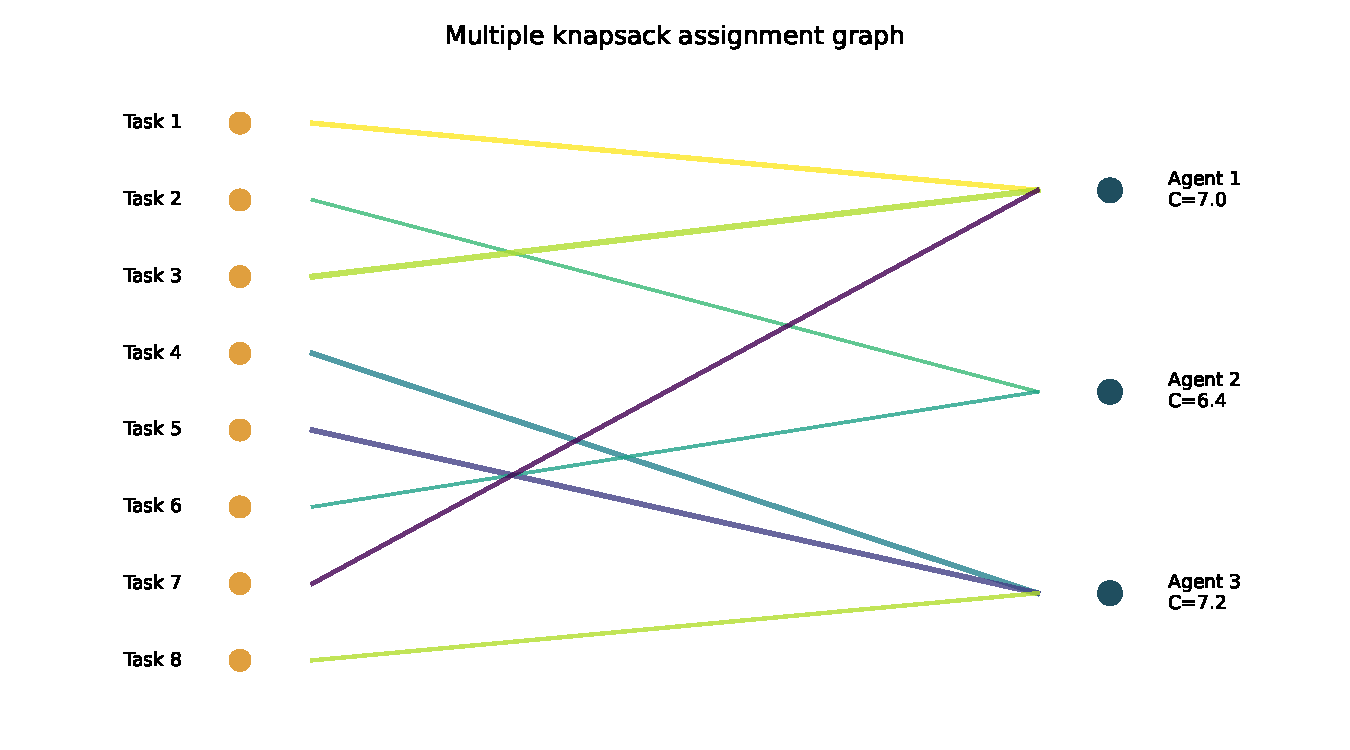
\includegraphics[width=0.7\textwidth]{mkp_structure.pdf}\par
	\vspace{0.2cm}
	\begin{minipage}{0.7\textwidth}
		\selectfont\tiny Bipartite assignment: tasks (left) are assigned to agents (right) with
				capacities $C_j$.  Edge width encodes task size $\E[S_{ij}]$ and color
				indicates expected return $R_{ij}$.  Each task is assigned to at most
				one agent (constraint~\ref{eq:assign}).
	\end{minipage}
\end{frame}

\begin{frame}{Stochastic Sizes and Returns}
	\centering
	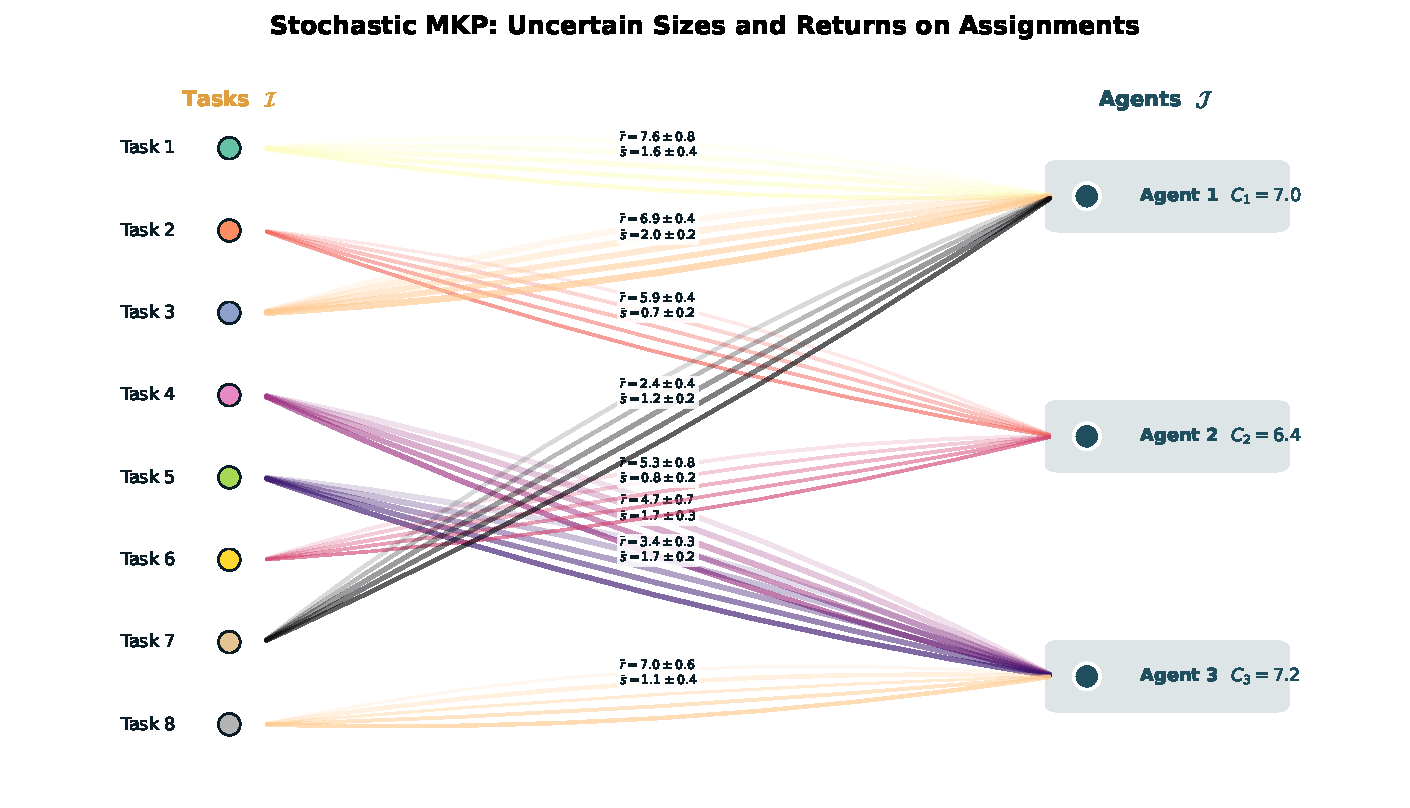
\includegraphics[width=0.7\textwidth]{mkp_stochastic.pdf}\par
	\vspace{0.2cm}
	\begin{minipage}{0.7\textwidth}
		\selectfont\tiny Stochastic extensions: each assignment edge shows multiple scenario
		realizations of size $S_{ij}^\omega$ (line width) and return $R_{ij}$ (annotation).
		The chance constraint~\eqref{eq:chance} limits the probability that total
		realized load exceeds agent capacity.
	\end{minipage}
\end{frame}

\section{Methodological Context}

\begin{frame}{Stochastic Knapsack: Cutting Planes and Dominance}
	\begin{itemize}
		\item \citet{büyüktahtakın_scenario_2023} derive \textbf{scenario dominance cuts} for multi-stage
			\textcolor{red}{stochastic MIPs} applied to the dynamic multi-dimensional knapsack.
			Strong dominance cuts reduce solution time with 0.06\% average deviation
			from optimality.
		\item \citet{büyüktahtakın_stage_2022} generalize this via \textbf{Stage-$t$ Scenario Dominance}
			for risk-averse (mean-CVaR) knapsack problems, achieving one-to-two
			orders of magnitude speedup.
		\item \citet{joung_comparative_2023} \textcolor{red}{compare LP relaxation bounds} for the robust knapsack
			problem and show that extended formulations yield identical bounds.
	\end{itemize}
\end{frame}

\begin{frame}{Distributionally Robust and Risk-averse Knapsack}
	\begin{itemize}
		\item \citet{bos_distributionally_2024} approximate the stochastic knapsack with periodic
			scheduled arrivals using \textbf{Wasserstein Distributed Robust Optimization (DRO)}, producing robust healthcare
			surgical schedules.
		\item \citet{ding_balancing_2022} propose a target-based DRO knapsack with
			\textbf{uncertain profit and capacity}, reformulated as a \textcolor{red}{second-order conic program}.
		\item \citet{merzifonluoglu_risk_2021} study the \textbf{risk-averse static stochastic knapsack}
			with CVaR and mean-standard deviation objectives, deriving efficient
			heuristics for normally distributed resource consumption.
		\item \citet{boonstra_robust_2025} solve a robust multi-item newsvendor with budget
			constraint using a greedy knapsack algorithm under moment ambiguity.
	\end{itemize}
\end{frame}

\begin{frame}{Solution Algorithms for Stochastic Programs}
	\begin{itemize}
		\item \citet{chen_sample_2022} analyze \textbf{sample average approximation} for two-stage
			programs without complete recourse, proving exponential convergence of
			recourse likelihood.
		\item \citet{larsen_fast_2024} accelerate L-shaped methods via \textbf{supervised ML},
			solving stochastic multi-knapsack instances in 20\% of the time with
			less than 0.1\% optimality gap.
		\item \citet{lefebvre_adjustable_2024} reformulate adjustable robust optimization with
			\textbf{discrete uncertainty} and apply \textcolor{red}{branch-and-cut to the multiple
			knapsack problem with uncertain weights}.
		\item \citet{lyu_stochastic_2022} unify \textcolor{red}{responsive, adaptive, and anticipative allocation
			policies} for the stochastic knapsack through \textbf{persistency values}.
	\end{itemize}
\end{frame}

\begin{frame}{Assignment, Scheduling, and Workforce Planning}
	\begin{itemize}
		\item \citet{rezaeian_assignment_2024} model the \textbf{stochastic assignment of projects} to
			managers via \textcolor{red}{multi-stage stochastic integer programming} with heuristic
			algorithms for large instances.
		\item \citet{nasirian_multiskilled_2025} solve multiskilled workforce staffing and scheduling
			via \textbf{logic-based Benders decomposition}, achieving 29x speedup over
			direct MILP solving.
		\item \citet{cavagnini_workforce_2020} use two-stage stochastic programming for production
			planning under \textbf{uncertain learning rates}, with insights on
			cross-training and worker assignment.
		\item \citet{novak_scheduling_2022} connect stochastic parallel machine scheduling to an
			\textbf{inflatable stochastic knapsack} pricing subproblem within
			\textcolor{red}{branch-and-price}.
	\end{itemize}
\end{frame}

\section{Benders Decomposition}

\begin{frame}{Why Benders Decomposition?}
	\begin{itemize}
		\item<1-> The full formulation carries one binary variable $y_j^\omega$ and
			one capacity constraint per agent-scenario pair.
		\item<2-> As the number of agents, tasks, and scenarios grows,
			solving the compact model directly becomes expensive.
		\item<3-> \textbf{Key insight}: the scenario-based chance constraints
			can be checked \emph{after} a candidate assignment is fixed.
		\item<4-> Benders decomposition separates the problem into:
			\begin{itemize}
				\item A \textbf{master problem} that decides assignments and
					evaluates the return-balance trade-off.
				\item A \textbf{feasibility subproblem} that checks whether the
					candidate assignment satisfies chance constraints.
			\end{itemize}
		\item<5-> This mirrors the managerial logic: propose an assignment
			first, then verify safety under uncertainty.
	\end{itemize}
\end{frame}

\begin{frame}{Benders Decomposition: Key Idea}
	\onslide<1->{%
	Given a program with complicating variables $y \in Y$ and
	easy variables $x \geq 0$, Benders decomposition reformulates
	it as a master problem over $y$ alone:}
	\onslide<2->{%
	\[
		\min_{y \in Y} \; z + d'y
	\]}
	\onslide<3->{%
	\vspace{-0.3cm}
	subject to \textbf{optimality cuts} (from dual extreme points
	$\pi_p$, $p \in \mathcal{P}$):
	\[
		z \;\geq\; \pi_p'(e - By), \quad \forall p \in \mathcal{P}
	\]}
	\onslide<4->{%
	\vspace{-0.3cm}
	and \textbf{feasibility cuts} (from dual extreme rays
	$\rho_r$, $r \in \mathcal{R}$):
	\[
		\rho_r'(e - By) \leq 0, \quad \forall r \in \mathcal{R}
	\]}
	\onslide<5->{%
	Cuts are generated iteratively rather than enumerated.
	Convergence is finite because the dual polyhedron has finitely
	many extreme points and rays.}
\end{frame}

\begin{frame}{Our Decomposition Structure}
	\onslide<1->{%
	\textbf{Notation.} Define the expected workload coefficient:
	\[
		\bar{S}_{ij} = \sum_{\omega \in \Omega} p_\omega\, S_{ij}^\omega,
		\quad \forall i \in \mathcal{I},\; \forall j \in \mathcal{J}.
	\]}
	\onslide<2->{%
	The utilization then simplifies to:
	\[
		U_j = \frac{1}{C_j}\sum_{i \in \mathcal{I}} \bar{S}_{ij}\, x_{ij},
		\quad \forall j \in \mathcal{J}.
	\]}
	\onslide<3->{%
	\begin{itemize}
		\item The \textbf{workload-balance component} depends only on expected
			workload, so it stays in the master problem.
		\item The \textbf{scenario-based chance feasibility} is naturally
			evaluated only after a candidate assignment is fixed.
	\end{itemize}}
\end{frame}

\begin{frame}{Master Problem (Iteration $t$)}
	Let $\mathcal{B}^t$ denote the set of feasibility cuts generated so far.
	\onslide<1->{%
	\[\max_{x,U,Z} \quad
		\sum_{j}\sum_{i} R_{ij}\, x_{ij}
		\;-\; \lambda\, Z
		\quad \text{(MP-Obj)}\label{eq:mp-obj}
	\]}
	\onslide<2->{%
	\vspace{-0.5cm}
	\[\text{s.t.} \quad \sum_{j} x_{ij} \leq 1,
		\quad \forall i \quad \text{(MP-1)}
	\]}
	\onslide<3->{%
	\vspace{-0.5cm}
	\[U_j = \tfrac{1}{C_j}\textstyle\sum_{i}
		\bar{S}_{ij}\, x_{ij},
		\quad \forall j \quad \text{(MP-2)}
	\]}
	\onslide<4->{%
	\vspace{-0.5cm}
	\[U_j - U_k \leq Z,
		\quad \forall j,k \quad \text{(MP-3)}
	\]}
	\onslide<5->{%
	\vspace{-0.5cm}
	\[x \in \mathcal{B}^t \quad \text{(MP-4)}
	\]}
	\onslide<6->{%
	\vspace{-0.1cm}
	\small The master keeps the true objective and balance structure.
	Chance constraints are \emph{not} included here; they are checked
	in the feasibility subproblem.}
\end{frame}

\begin{frame}{Feasibility Evaluation Subproblem}
	Given a candidate assignment $\bar{x}$ from the master:
	\begin{itemize}
		\item<1-> \textbf{Step 1.} Compute realized workload in each scenario:
			\[
				L_j^\omega(\bar{x}) = \sum_{i \in \mathcal{I}}
				S_{ij}^\omega\, \bar{x}_{ij},
				\quad \forall j,\; \forall \omega.
			\]
		\item<2-> \textbf{Step 2.} Determine scenario violations:
			\[
				\delta_j^\omega(\bar{x}) =
				\begin{cases}
					1, & \text{if } L_j^\omega(\bar{x}) > C_j,\\
					0, & \text{otherwise.}
				\end{cases}
			\]
		\item<3-> \textbf{Step 3.} Compute violation probability:
			\[
				P_j^{\text{viol}}(\bar{x}) = \sum_{\omega \in \Omega}
				p_\omega\, \delta_j^\omega(\bar{x}).
			\]
		\item<4-> \textbf{Step 4.} Check: $\bar{x}$ is chance-feasible if and only if
			$P_j^{\text{viol}}(\bar{x}) \leq \alpha$ for all $j \in \mathcal{J}$.
	\end{itemize}
	\onslide<5->{%
	\vspace{0.1cm}
	\small This is a \textbf{logical feasibility check}, not another optimization
	problem. Once $\bar{x}$ is fixed, all quantities are computed directly.}
\end{frame}

\begin{frame}{Feasibility Cut Generation}
	If agent $j$ violates the chance constraint under $\bar{x}$:
	\begin{itemize}
		\item<1-> Let $\mathcal{I}_j(\bar{x}) = \{i \in \mathcal{I} : \bar{x}_{ij} = 1\}$
			be the tasks assigned to agent $j$.
		\item<2-> \textbf{No-good cut}: prevent reassigning the exact same bundle:
			\[
				\sum_{i \in \mathcal{I}_j(\bar{x})} x_{ij}
				\;\leq\; |\mathcal{I}_j(\bar{x})| - 1.
			\]
		\item<3-> \textbf{Stronger cut}: identify a minimal offending subset
			$\mathcal{B}_j(\bar{x}) \subseteq \mathcal{I}_j(\bar{x})$ such that
			\[
				\sum_{\omega \in \Omega:\,
				\sum_{i \in \mathcal{B}_j} S_{ij}^\omega > C_j}
				p_\omega \;>\; \alpha.
			\]
		\item<4-> Then add the tighter cut:
			\[
				\sum_{i \in \mathcal{B}_j(\bar{x})} x_{ij}
				\;\leq\; |\mathcal{B}_j(\bar{x})| - 1.
			\]
			This excludes the specific offending combination while leaving
			more flexibility for the master.
	\end{itemize}
\end{frame}

\begin{frame}{Algorithm: Step-by-Step}
	\begin{enumerate}
		\item<1-> \textbf{Initialize.} Set $t = 0$, $\mathcal{B}^0 = \emptyset$.
		\item<2-> \textbf{Solve Master Problem.}
			Solve~\eqref{eq:mp-obj} to obtain candidate $\bar{x}$.
		\item<3-> \textbf{Feasibility Check.}
			For each agent $j$, compute $L_j^\omega(\bar{x})$ in every scenario
			and evaluate $P_j^{\text{viol}}(\bar{x})$.
		\item<4-> \textbf{If feasible} ($P_j^{\text{viol}} \leq \alpha$ for all $j$):
			$\bar{x}$ is optimal. \textbf{Stop.}
		\item<5-> \textbf{If infeasible}: for each violating agent $j$,
			generate a feasibility cut and add it to $\mathcal{B}^{t+1}$.
		\item<6-> \textbf{Update.} Set $t \leftarrow t + 1$. Return to Step~2.
	\end{enumerate}
	\onslide<7->{%
	\vspace{0.2cm}
	\begin{block}{Convergence}
		The algorithm terminates in finitely many iterations because
		each feasibility cut eliminates at least one infeasible
		assignment pattern, and the number of binary assignment
		patterns is finite.
	\end{block}}
\end{frame}

\begin{frame}{Why This Decomposition Works}
	\begin{itemize}
		\item<1-> \textbf{Exact objective in master}: every master solution is
			evaluated with respect to the exact return-balance trade-off.
		\item<2-> \textbf{Scenario-free master}: all agent-scenario binary variables
			$y_j^\omega$ are removed from the main optimization.
		\item<3-> \textbf{Simple subproblem}: the feasibility check is
			purely arithmetic (no LP or MIP to solve).
		\item<4-> \textbf{Managerial interpretation}: the planner proposes an
			assignment, then checks whether it is sufficiently safe under
			workload uncertainty.
	\end{itemize}
\end{frame}

\section{Computational Results}

\begin{frame}{Test Instances}
	Three instances with increasing size:
	\vspace{0.2cm}
	\begin{center}
	\begin{tabular}{lccccc}
		\toprule
		Instance & Tasks & Agents & Scenarios & $\alpha$ & $\lambda$ \\
		\midrule
		Small  & 5  & 3  & 3  & 0.20 & 4.0 \\
		Medium & 10 & 5  & 5  & 0.20 & 5.0 \\
		Large  & 25 & 10 & 10 & 0.10 & 6.0 \\
		\bottomrule
	\end{tabular}
	\end{center}
	\pause
	\vspace{0.2cm}
	\begin{itemize}
		\item Capacities vary slightly across agents
			(e.g., $[10, 10, 11]$ for the small instance).
		\item The large instance uses a tighter risk tolerance ($\alpha = 0.10$).
	\end{itemize}
\end{frame}

\begin{frame}{Computational Summary}
	\begin{center}
	\begin{tabular}{lcccccc}
		\toprule
		Instance & Objective & Return & $Z$ & Iterations & Cuts & Gap \\
		\midrule
		Small  & 51.50  & 53  & 0.376 & 2   & 1    & 0.00 \\
		Medium & 77.11  & 79  & 0.377 & 52  & 220  & 0.00 \\
		Large  & 254.34 & 257 & 0.444 & 443 & 1958 & 0.00 \\
		\bottomrule
	\end{tabular}
	\end{center}
	\pause
	\vspace{0.2cm}
	\begin{itemize}
		\item All instances close the Benders gap to zero.
		\item The number of iterations and cuts increases substantially with
			instance size: from 2 iterations / 1 cut (small) to
			443 iterations / 1958 cuts (large).
	\end{itemize}
\end{frame}

\begin{frame}{Small Instance: Assignment and Utilization}
	\begin{columns}[T]
		\begin{column}{0.48\textwidth}
			\onslide<1->{%
			\textbf{Assignment}
			\begin{center}
			\begin{tabular}{ll}
				\toprule
				Task & Agent \\
				\midrule
				1 & Agent 3 \\
				2 & Agent 2 \\
				3 & Agent 3 \\
				4 & Agent 2 \\
				5 & Agent 1 \\
				\bottomrule
			\end{tabular}
			\end{center}}
		\end{column}
		\begin{column}{0.48\textwidth}
			\onslide<2->{%
			\textbf{Expected utilization}
			\begin{center}
			\begin{tabular}{lc}
				\toprule
				Agent & $U_j$ \\
				\midrule
				1 & 0.570 \\
				2 & 0.940 \\
				3 & 0.946 \\
				\bottomrule
			\end{tabular}
			\end{center}}
		\end{column}
	\end{columns}
	\onslide<3->{%
	\vspace{0.3cm}
	\begin{itemize}
		\item Solved in 2 iterations with 1 feasibility cut.
		\item The first master solution was infeasible because agent 1 received
			an unsafe bundle. One cut corrected this.
	\end{itemize}}
\end{frame}

\begin{frame}{Medium Instance: Assignment and Utilization}
	\begin{columns}[T]
		\begin{column}{0.48\textwidth}
			\onslide<1->{%
			\textbf{Assignment}
			\begin{center}
			\begin{tabular}{ll}
				\toprule
				Task & Agent \\
				\midrule
				2  & Agent 2 \\
				3  & Agent 3 \\
				4  & Agent 4 \\
				5  & Agent 5 \\
				7  & Agent 1 \\
				10 & Agent 4 \\
				\bottomrule
			\end{tabular}
			\end{center}
			\small Tasks 1, 6, 8, 9: \textbf{not assigned}.}
		\end{column}
		\begin{column}{0.48\textwidth}
			\onslide<2->{%
			\textbf{Expected utilization}
			\begin{center}
			\begin{tabular}{lc}
				\toprule
				Agent & $U_j$ \\
				\midrule
				1 & 0.545 \\
				2 & 0.628 \\
				3 & 0.545 \\
				4 & 0.922 \\
				5 & 0.645 \\
				\bottomrule
			\end{tabular}
			\end{center}}
		\end{column}
	\end{columns}
	\onslide<3->{%
	\vspace{0.2cm}
	\begin{itemize}
		\item 52 iterations and 220 feasibility cuts.
		\item Leaving some tasks unassigned is optimal: assigning them would
			violate chance constraints or create too much imbalance.
	\end{itemize}}
\end{frame}

\begin{frame}{Large Instance: Assignment and Utilization}
	\begin{columns}[T]
		\begin{column}{0.48\textwidth}
			\onslide<1->{%
			\textbf{Assignment highlights}
			\begin{itemize}
				\item 19 of 25 tasks are assigned.
				\item Tasks 5, 11, 12, 17, 23, 24: not assigned.
				\item Most agents receive 2 tasks;
					agent 7 receives only 1.
			\end{itemize}}
		\end{column}
		\begin{column}{0.48\textwidth}
			\onslide<2->{%
			\textbf{Expected utilization}
			\begin{center}
			\footnotesize
			\begin{tabular}{lc}
				\toprule
				Agent & $U_j$ \\
				\midrule
				1  & 0.786 \\
				2  & 0.722 \\
				3  & 0.730 \\
				4  & 0.722 \\
				5  & 0.739 \\
				6  & 0.747 \\
				7  & 0.355 \\
				8  & 0.748 \\
				9  & 0.785 \\
				10 & 0.755 \\
				\bottomrule
			\end{tabular}
			\end{center}}
		\end{column}
	\end{columns}
	\onslide<3->{%
	\vspace{0.1cm}
	\small 443 iterations and 1958 cuts. Feasible but not perfectly
	balanced. Agent 7 is the lightest outlier.}
\end{frame}

\begin{frame}{Observations from Results}
	\begin{itemize}
		\item<1-> \textbf{Scalability}: iterations and cuts grow substantially
			with instance size (from 2 to 443 iterations).
		\item<2-> \textbf{Not all tasks are assigned}: the optimizer leaves
			tasks undone when assigning them would violate chance constraints
			or worsen imbalance.
		\item<3-> \textbf{Workload balance}: the balance penalty $\lambda Z$
			keeps utilization spread moderate, though perfect balance is
			not always achievable.
		\item<4-> \textbf{Zero Benders gap}: all instances are solved to
			proven optimality, confirming correctness of the decomposition.
		\item<5-> \textbf{Computational cost}: the explicit outer-loop
			Benders scheme becomes expensive for large instances with
			tight chance constraints, suggesting room for acceleration
			strategies.
	\end{itemize}
\end{frame}

\section{Takeaways}

\begin{frame}{Key Takeaways}
	\begin{itemize}
		\item<1-> The formulation models cognitive resource allocation as a
			\textbf{stochastic multiple knapsack} with scenario-based chance
			constraints and a workload-balance penalty.
		\item<2-> \textbf{Benders decomposition} separates assignment decisions
			from chance-feasibility checks, keeping the exact objective in
			the master and using a simple logical subproblem.
		\item<3-> Computational results on three instances demonstrate
			correctness (zero gap) and reveal the scalability challenge
			as instance size grows.
		\item<4-> Future directions include stronger cut generation,
			scenario dominance \citep{büyüktahtakın_scenario_2023},
			and ML-accelerated decomposition \citep{larsen_fast_2024}.
	\end{itemize}
\end{frame}

\section{References}

\begin{frame}[allowframebreaks]{References}
	\bibliographystyle{plainnat}
	\bibliography{../literature/reference,../Formulation/Literature/SImilar40/knapsack_20260209_165848}
\end{frame}

\end{document}
